% =================================================================================================
% File:			appendici.tex
% Description:	Definisce le appendici riguardanti gli standard di qualità
% Created:		2014/01/11
% Author:		Ceccon Lorenzo
% Email:		ceccon.lorenzo@mashup-unipd.it
% =================================================================================================
% Modification History:
% Version		Modifier Date		Change											Author
% 0.0.1 		2014/01/11 			iniziata stesura appendice					Lorenzo C.
% =================================================================================================
%% Version		Modifier Date		Change											Author
% 1.0.1 		2015/03/17 			iniziata stesura appendice B				Nicola F.
% =================================================================================================
%


% CONTENUTO DEL CAPITOLO

\appendix 

\section{Modelli e standard di qualità}
  	\subsection{Standard ISO/IEC 9126}
  	Lo standard ISO/IEC 9126 è uno standard creato per delineare delle normative utili a descrivere un modello di qualità del software. Lo standard propone un approccio in cui viene posta attenzione al miglioramento dell'organizzazione e dei processi di una società di software, in modo da migliorare di conseguenza la qualità del prodotto software.\\
  	\begin{figure}[h]
		\centering
		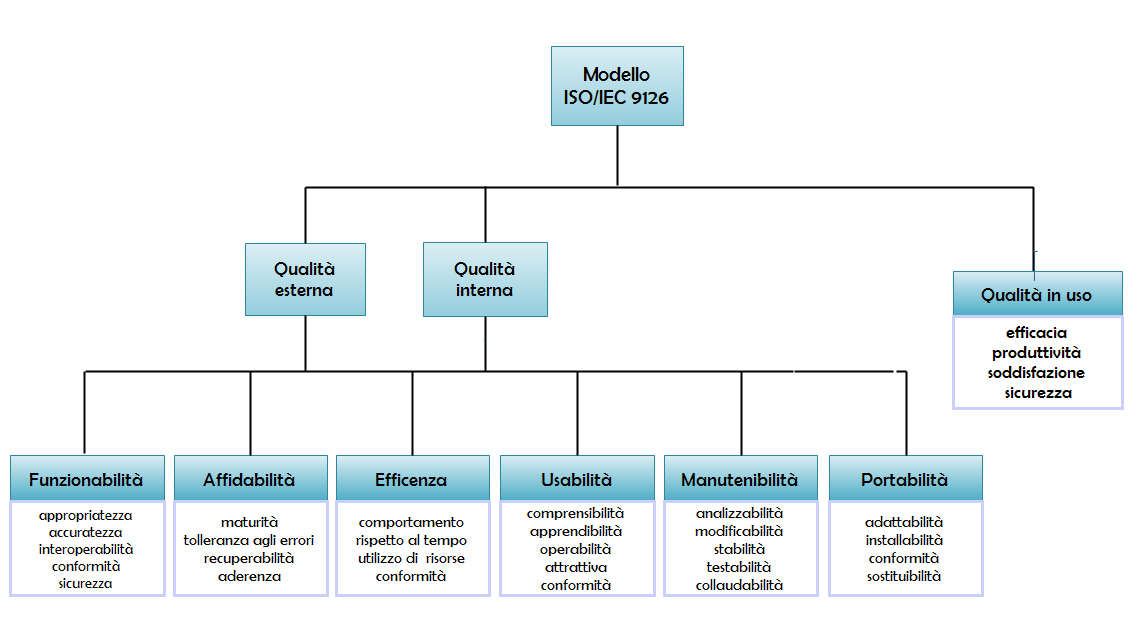
\includegraphics[width=140mm]{images/iso_9126.png}
		\caption{Schema del modello di qualità ISO/IEC 9126}
		\label{fig:iso9126}
	\end{figure}
  	Lo standard ISO/IEC 9126 è suddiviso in quattro parti:
		\begin{itemize}
			\item \textbf{Modello di qualità: } la prima parte dello standard classifica il modello di qualità in sei caratteristiche generali e in varie sotto caratteristiche misurabili tramite l'utilizzo di metriche.\\
			Le sei caratteristiche generali e le relative sotto caratteristiche sono:
				\begin{itemize}
					\item \textbf{Funzionalità:} capacità di un prodotto software di fornire funzioni che soddisfano esigenze stabilite
						\begin{itemize}
							\item \textbf{Appropriatezza:} capacità del prodotto software di fornire un appropriato insieme di funzioni per i specifici compiti ed obiettivi prefissati all'utente;
							\item \textbf{Accuratezza:} capacità del prodotto software di fornire i risultati richiesti;
							\item \textbf{Interoperabilità:} capacità del prodotto software di interagire con i diversi sistemi specificati;
							\item \textbf{Conformità:} capacità del prodotto software di aderire agli standard e alle convenzioni appartenenti al settore in cui vengono applicati;
							\item \textbf{Sicurezza:} capacità del prodotto software di consentire l'accesso a dati e informazioni solamente alle persone autorizzate.
						\end{itemize}
					\item \textbf{Affidabilità:} capacità del prodotto software di mantenere uno specificato livello di prestazioni
						\begin{itemize}
							\item \textbf{Maturità:} capacità di un software di evitare che si verificano errori, malfunzionamenti o siano prodotti risultati non corretti;
							\item \textbf{Tolleranza agli errori:} capacità del software di mantenere un adeguato livello di prestazioni in presenza di malfunzionamenti;
							\item \textbf{Recuperabilità:} capacità di un prodotto di ripristinare il livello appropriato di prestazioni in seguito a un malfunzionamento;
							\item \textbf{Aderenza:} capacità di aderire a standard, regole e convenzioni inerenti all'affidabilità.
						\end{itemize}
					\item \textbf{Usabilità:} capacità del software di essere capito, appreso e usato dall'utente
						\begin{itemize}
							\item \textbf{Comprensibilità:} esprime la facilità di comprensione delle funzionalità del prodotto;
							\item \textbf{Apprendibilità:} capacità del software di essere appreso in tempo brevi;
							\item \textbf{Operabilità:} capacità di permettere agli utenti di utilizzare al software al fine di raggiungere i propri scopi;
							\item \textbf{Attrattiva:} capacità del prodotto di risultare interessante all'utente;
							\item \textbf{Conformità:} capacità del software di aderire a standard, regole e convenzioni relativi all'usabilità.
						\end{itemize}
					\item \textbf{Efficienza:} capacità di fornire prestazioni relativamente alla quantità di risorse usate
						\begin{itemize}
							\item \textbf{Comportamento rispetto al tempo:} capacità di fornire tempi di risposta, elaborazione e velocità di attraversamento ottimali in relazione alla funzione utilizzata;
							\item \textbf{Utilizzo delle risorse:} capacità del software di utilizzare adeguate quantità di risorse;
							\item \textbf{Conformità:} capacità del software di aderire a standard, regole e convenzioni relativi all'efficienza.
						\end{itemize}
					\item \textbf{Manutenibilità:} capacità del software di essere modificato apportando correzioni, miglioramenti o adattamenti
						\begin{itemize}
							\item \textbf{Analizzabilità:} esprime la facilità nell'analizzare il codice sorgente per ricercare errori; 
							\item \textbf{Modificabilità:} capacità del software di permettere l'implementazione di nuove modifiche;
							\item \textbf{Stabilità:} capacità del software di evitare effetti indesiderati a seguito di modifiche errate;
							\item \textbf{Testabilità:} capacità del software di eseguire facilmente la validazione delle modifiche apportate al software.
						\end{itemize}
					\item \textbf{Portabilità:} capacità del software di lavorare in diversi ambienti di lavoro
						\begin{itemize}
							\item \textbf{Adattabilità:} capacità del software di essere adattato a diversi ambienti senza dover applicare modifiche diverse da quelle fornite;
							\item \textbf{Installabilità:} capacità del software di essere installato in uno specificato ambiente;
							\item \textbf{Conformità:} capacità del prodotto software di aderire a standard, regole e convenzioni relativi alla portabilità;
							\item \textbf{Sostituibilità:} capacità del software di sostituire un altro software analogo per svolgere certi compiti.
						\end{itemize}
				\end{itemize}
			\item \textbf{Qualità esterne: } le metriche esterne applicabili al software, e quindi rilevabili tramite l'analisi dinamica, misurano i comportamento del prodotto sulla base dei test, dall'operatività e dall'osservazione durante la sua esecuzione;
			\item \textbf{Qualità interne: } le metriche interne, misurabili attraverso l'analisi statica, sono utili per prevedere il livello della qualità esterna ed in uso, poiché i suoi attributi interni influiscono su quelli esterni ed in uso. Permettono così di individuare anomalie prima che queste ultime possano influenzare la qualità del prodotto finale;
			\item \textbf{Qualità in uso: } la qualità in uso, raggiungibile solo dopo aver ottenuto la qualità interna ed esterna, fornisce metriche per misurare il grado di utilizzabilità del prodotto da parte dell'utente finale.
		\end{itemize}
		
	\subsection{Standard ISO/IEC 15504}
	Lo standard ISO/IEC 15504, conosciuto anche come SPICE, è un insieme di documenti tecnici per lo sviluppo di processi software, utili a valutare la dimensione dei processi tramite l'utilizzo di specifiche metriche. É derivato dallo standard ISO/IEC 12207 e da modelli di maturità quali Bootstrap, Trillium e il CMM.\\
	Lo standard definisce la dimensione del processo e la suddivide nelle seguenti cinque categorie:
		\begin{itemize}
			\item \textbf{Custormer/Supplier;}
			\item \textbf{Engineering;}
			\item \textbf{Support;}
			\item \textbf{Management;}
			\item \textbf{Organization.}
		\end{itemize}
	Per ogni processo, viene definito un livello di capacità dei processi definito da una scala di sei livelli e da nove attributi suddivisi nei vari livelli:
		\begin{itemize}
			\item \textbf{Level 5. Optimizing process:} il processo è predicibile ed in grado di adattarsi per raggiungere
obiettivi specifici
				\begin{itemize}
					\item \textbf{Process Innovation:} le modifiche ad un processo sono identificate ed implementate al fine di ottenere il miglioramento continuo nel raggiungimento degli obiettivi;
					\item \textbf{Process Optimization:} le modifiche alla definizione, gestione, attuazione di un processo sono controllate.
				\end{itemize}
			\item \textbf{Level 4. Predictable process:} il processo è stabilizzato ed è attuato all'interno di definiti limiti di controllo
				\begin{itemize}
					\item \textbf{Process Measurement:} i risultati raggiunti e le misure rilevate durante l'attuazione di un processo sono utilizzati per garantire il raggiungimento di specifici obiettivi;
					\item \textbf{Process Control:} un processo è controllato attraverso le misure di prodotto e di processo rilevate, al fine di migliorare le modalità di attuazione del processo stesso.
				\end{itemize}
			\item \textbf{Level 3. Established process:} il processo è attuato, pianificato e controllato sulla base di procedure standard basate sui principi dell'ingegneria del software
				\begin{itemize}
					\item \textbf{Process Definition:} l'attuazione di un processo, per raggiungere gli obiettivi, si basa sull'adozione di approcci standard;
					\item \textbf{Process Deployment:} l'attuazione di un processo, per raggiungere gli obiettivi, fa uso di risorse umane e tecniche appropriate.
				\end{itemize}
			\item \textbf{Level 2. Managed process:} il processo è attuato ma anche pianificato, tracciato, verificato ed aggiustato se necessario, sulla base di obiettivi ben definiti
				\begin{itemize}
					\item \textbf{Performance Management:} l'implementazione di un processo è pianificato e controllato al fine di produrre risultati coerenti agli obiettivi attesi;
					\item \textbf{Work Product Management:} l'implementazione di un processo è pianificato e controllato al fine di produrre risultati documentati, controllati e verificati in modo appropriato.
				\end{itemize}			
			\item \textbf{Level 1. Performed process:} il processo viene messo in atto e raggiunge i suoi obiettivi. Il risultato potrebbe non essere stato pianificato e tracciato rigorosamente
				\begin{itemize}
					\item \textbf{Process Performance:} capacità di un processo di raggiungere i suoi obiettivi trasformando input identificabili in output identificabili.
				\end{itemize}
			\item \textbf{Level 0. Incomplete process:} il processo non è stato implementato oppure non raggiunge gli obiettivi.
		\end{itemize}
	Ogni attributo è misurabile tramite l'utilizzo di una scala di valutazione divisa in quattro punti:
		\begin{itemize}
			\item \textbf{Not achieved (0-15\%);}
			\item \textbf{Partially achieved (15-50\%);}
			\item \textbf{Largely achieved (50-85\%);}
			\item \textbf{Fully achieved (85-100\%).}
		\end{itemize}
	Lo standard fornisce una guida per l'effettuazione di una valutazione formata da:
		\begin{itemize}
			\item Processo di valutazione;
			\item Modello per la valutazione;
			\item Strumenti per la valutazione.
		\end{itemize}
	Lo standard infine, stabilisce che per una corretta valutazione i verificatori debbano avere un buon livello di competenza e di esperienza.
	
	\subsection{Ciclo PDCA}
	Il ciclo PDCA, noto anche come ciclo di Deming, è un metodo di gestione iterativo a quattro fasi per il controllo e il miglioramento continuo dei processi.\\
	Le quattro fasi che lo compongono sono:
			\begin{itemize}
				\item \textbf{Plan:} stabilisce gli obiettivi e i processi necessari per ottenere risultati uguali a quelli attesi;
				\item \textbf{Do:} fase composta dall'attuazione del piano, dall'esecuzione del processo e dalla creazione del prodotto. Termina con una raccolta dei dati e creazione di grafici sul risultato di quanto ottenuto;
				\item \textbf{Check:} si confrontano i risultati ottenuti dalla fase precedente con i risultati stabiliti durante la pianificazione per verificare la presenza di differenze;
				\item \textbf{Act:} si effettuano correzioni laddove sono presenti differenze tra i risultati ottenuti e quelli previsti. Si determinano le cause delle discrepanze e dove c'è bisogno di applicare delle modifiche per ottenere un miglioramento del processo e di conseguenza del prodotto.
			\end{itemize}
			\begin{figure}[h]
				\centering
				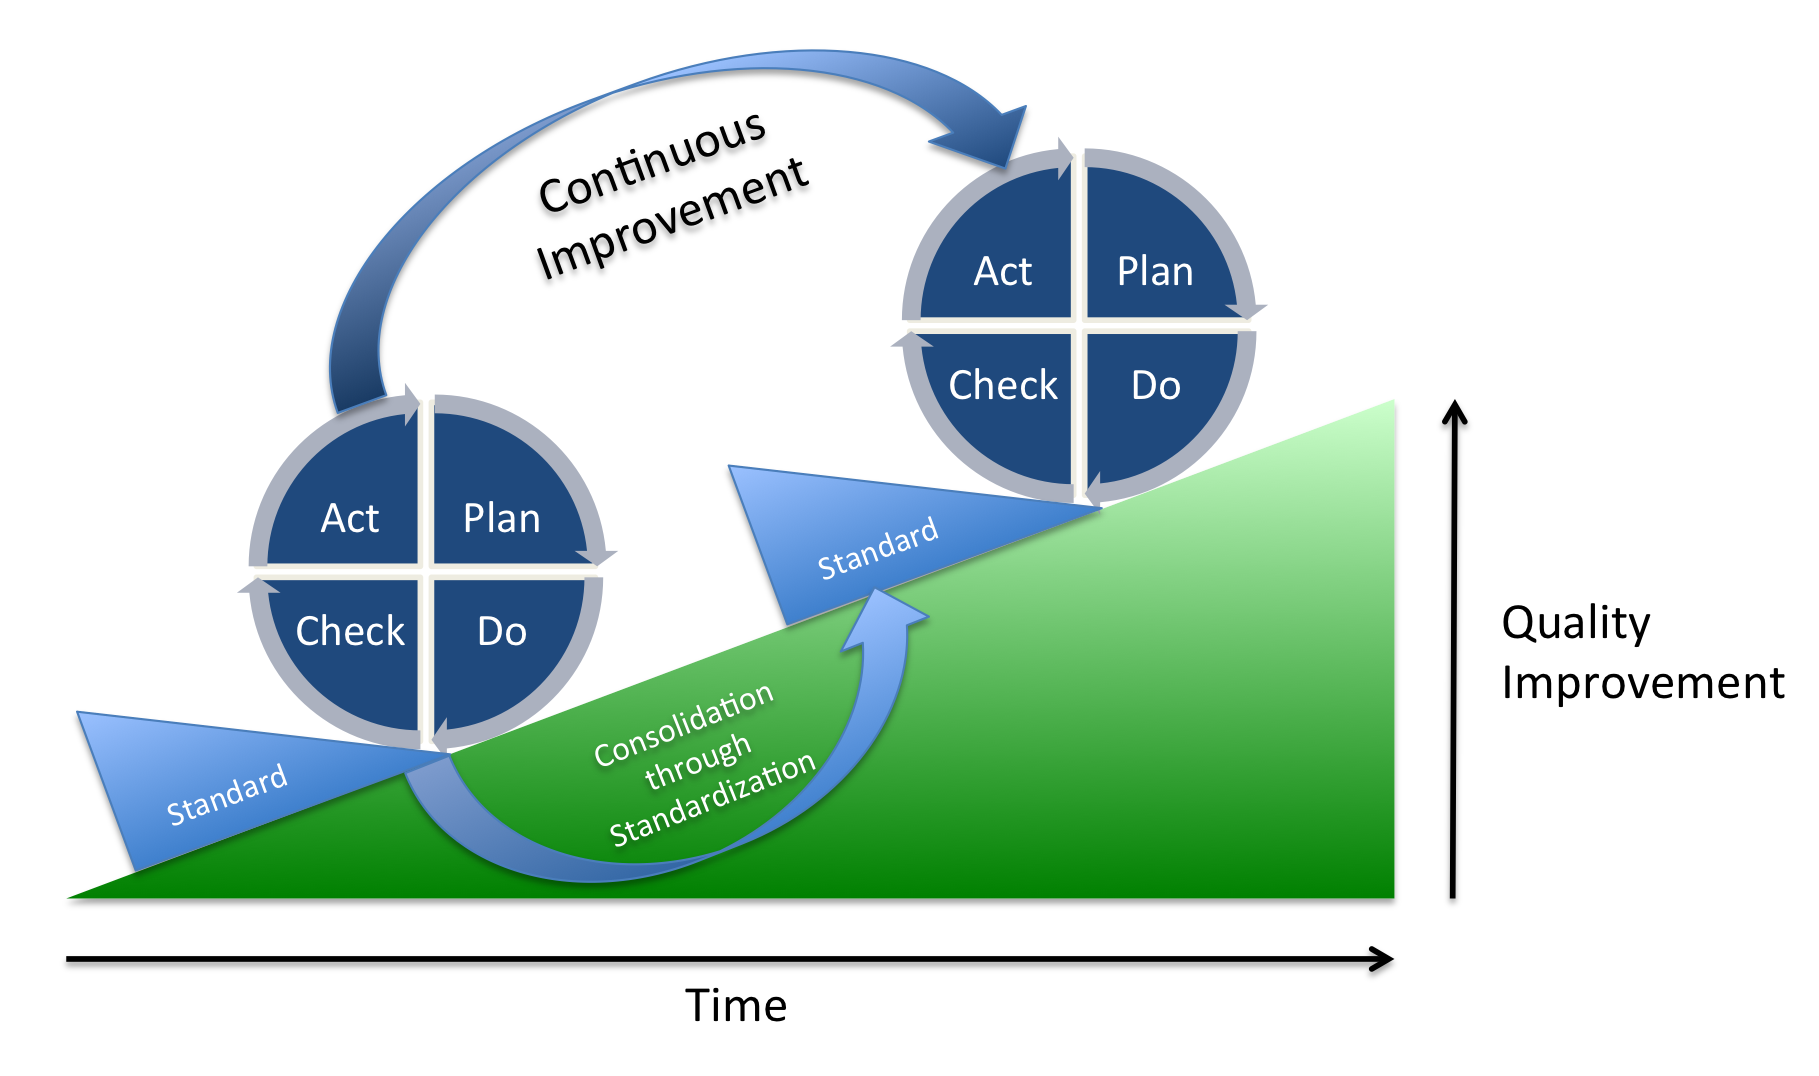
\includegraphics[width=120mm]{images/pdca.png}
				\caption{Ciclo di miglioramento della qualità PDCA}
				\label{fig:pdca}
			\end{figure}
		
\pagebreak

\section{Pianificazione dei test}
	\subsection{Descrizione test}
		In seguito sono descritti tutti i test di validazione, sistema e di integrazione pianificati. I test di unità invece verranno inseriti successivamente.
Lo stato \textbf{N.I.} presente nelle tabelle sottostanti è da intendersi come non applicato, tali test verranno infatti svolti successivamente come descritto in \docNameVersionPdP.\\
Per una descrizione più dettagliata sui test si rimanda alla sezione dei test del documento \docNameVersionNdP.

	\subsection{Test di sistema}
		I test di sistema servono per verificare che il sistema software completamente integrato soddisfi tutti i requisiti software individuati e descritti nel documento \docNameVersionAdR.
		\subsubsection{Descrizione dei test di sistema}
			\begin{center}

			\def\arraystretch{1.5}
			\bgroup
			\begin{longtable}{| p{2cm} | p{7cm} | p{1.5cm} | p{2cm} |}
					\hline
					\textbf{Test} & \textbf{Descrizione} & \textbf{Stato} & \textbf{Requisito}\\
					\hline						
					TSF1 & Viene verificato che il sistema permetta, all'utente non autenticato, la registrazione al servizio & N.I. & ROF1\\
					\hline
					TSF2 & Viene verificato che il sistema permetta all'utente di autenticarsi & N.I. & ROF2\\
					\hline
					TSF3 & Viene verificato che il sistema permetta, all'utente autenticato, di accedere al menù informazioni personali & N.I. & ROF3\\
					\hline
					TSF4 & Viene verificato che il sistema permetta, all'utente autenticato, di effettuare la deautenticazione & N.I. & ROF4\\
					\hline
					TSF5 & Viene verificato che il sistema permetta, all'utente autenticato, di visualizzare tutte le Recipe presenti nel sistema & N.I. & ROF5\\
					\hline
					TSF6 & Viene verificato che il sistema permetta all'utente di gestire le proprie View & N.I. & ROF6\\
					\hline
					TSF7 & Viene verificato che il sistema permetta di richiedere l'inserimento di una nuova Recipe & N.I. & ROF7\\
					\hline
					TSF8 & Viene verificato che il sistema permetta, all'utente amministratore autenticato, di accedere all'area riservata del sistema & N.I. & ROF8\\
					\hline
					TSF10 & Viene verificato che il sistema permetta, all'utente amministratore, di gestire la richiesta di nuove Recipe & N.I. & ROF10\\
					\hline
					TSF11 & Viene verificato che il sistema fornisca una serie di servizi REST & N.I. & ROF11\\
					\hline
					TSP1 & Viene verificato che l'utente visualizzi le proprie View entro 10 secondi & N.I. & RDP1\\
					\hline
					TSP2 & Viene verificato che l'interfaccia web utilizzi un design di tipo responsive & N.I. & RFP2\\
					\hline
					TSQ1 & Viene verificato che sia disponibile un manuale per l'utente & N.I. & ROQ1\\
					\hline
					TSQ2 & Viene verificato che tutto il codice rispetti le norme e le metriche descritte nel \docNameVersionPdQ{} e \docNameVersionNdP & N.I. & ROQ2\\
					\hline
					TSQ3 & Viene verificato che sia disponibile un manuale per l'uso dei servizi REST & N.I. & ROQ3\\
					\hline
					TSV1 & Viene verificato che il sistema utilizzi gli strumenti offerti da Google Cloud Platform & N.I. & RDV1\\
					\hline
					TSV2 & Viene verificato che il linguaggio di programmazione utilizzato per il server sia Python & N.I. & RDV2\\
					\hline
					TSV3 & Viene verificato che il codice soggetto sia soggetto a versionamento tramite il modello di branching descritto nelle \docNameVersionNdP & N.I. & RDV3\\
					\hline
					TSV4 & Viene verificato che l'interfaccia web sia di tipo single-page & N.I. & RDV4\\
					\hline
					TSV5 & Viene verificato che l'interfaccia web funzioni con i principali browser attualmente sul mercato& N.I. & ROV5\\
					\hline
					TSV6 & Viene verificato che il sistema utilizzi librerie esterne per effettuare le chiamate alle API dei diversi social network & N.I. & ROV6\\
					\hline
					TSV7 & Viene verificato che il sistema utilizzi librerie esterne per generare i grafici necessari alle View & N.I. & ROV7\\
					\hline
			\caption{Tracciamento test di sistema - requisiti}
			\end{longtable}
				\egroup
\end{center}
		
	\subsection{Test di integrazione}
		I test di integrazione vengono utilizzati per verificare che tutti i componenti del sistema siano integrati correttamente tra di loro e che il flusso dati all'interno del sistema sia corretto.\\
		Si è deciso di fare affidamento ad una strategia di integrazione di tipo incrementale in modo da permetterci di sviluppare e verificare più componenti in parallelo.\\
		La strategia incrementale ci permette anche di effettuare la ricerca dei difetti in maniera più precisa, infatti nel caso si presenti un errore, questo sarà probabilmente causato dall'ultima componente inserita e permettendoci di ritornare ad uno stato del sistema corretto.\\
		Viene utilizzato il metodo bottom-up, cioè vengono prima integrate le componenti con minor dipendenze funzionali e con maggiori funzionalità, che corrispondono, quindi, ai requisiti obbligatori. In questo modo è possibile ottenere un prodotto funzionante, che soddisfa tutti i requisiti obbligatori, il prima possibile. Sarà, quindi, necessario testare più volte le componenti per assicurarci che il prodotto software finale non contenga difetti.\\ Successivamente si procederà ad aggiungere le componenti che corrispondono ai requisiti desiderabili e opzionali.
		 
		\subsubsection{Descrizione dei test di integrazione}
			\begin{center}

			\def\arraystretch{1.5}
			\bgroup
			\begin{longtable}{| p{2.5cm} | p{5cm} | p{3.5cm} | p{1.5cm} |}
					\hline
					\textbf{Test} & \textbf{Descrizione} & \textbf{Componente} & \textbf{Stato}\\
					\hline						
					TO DO & TO DO & TO DO & TO DO\\
					\hline
			\caption{Tabella test di integrazione}
			\end{longtable}
				\egroup
\end{center}

	\subsection{Test di validazione}
		I test di validazione vengono utilizzati per accertarsi che il prodotto finale sviluppato sia conforme alle attese.\\
		Per ogni test viene riportata una descrizione contenente i passi che l'utente deve seguire per verificare che i requisiti siano soddisfatti. Il tracciamento tra test di validazione e i requisiti correlati viene riportati nel documento \docNameVersionAdR.
		
		\subsubsection{TVF1}
			L'utente vuole verificare che si possa registrare al sistema. All'utente è richiesto di:
			\begin{itemize}
				\item inserire un username;
				\item inserire una email;
				\item inserire una password;
				\item inserire una password di conferma;
				\item verificare che il sistema avverta l'utente in fase di compilazione se i dati inseriti non sono conformi alle norme del sistema;
				\item confermare la registrazione;
				\item verificare che il sistema avverta l'utente nel caso in cui i dati inseriti non siano conformi alle norme del sistema;
				\item verificare che, nel caso la registrazione abbia avuto esito positivo, venga inviata un email di conferma.
			\end{itemize}
			
		\subsubsection{TVF1.1}
			L'utente vuole verificare che l'inserimento di un username avvenga correttamente. All'utente è richiesto di:
			\begin{itemize}
				\item inserire un username;
				\item verificare che, se lo username è già presente nel database, venga visualizzato un errore;
				\item verificare che, nel caso lo username non sia conforme alle norme del sistema, venga visualizzato alcun errore.
			\end{itemize}
			
		\subsubsection{TVF1.2}
			L'utente vuole verificare che l'inserimento di una email avvenga correttamente. All'utente è richiesto di:
			\begin{itemize}
				\item inserire una email;
				\item verificare che, se la email è già presente nel database, venga visualizzato un errore;
				\item verificare che, nel caso la email non sia conforme alle norme del sistema, venga visualizzato un errore.
			\end{itemize}
			
		\subsubsection{TVF1.3}
			L'utente vuole verificare che l'inserimento di una password avvenga correttamente. All'utente è richiesto di:
			\begin{itemize}
				\item inserire una password;
				\item verificare che, nel caso la password non sia conforme alle norme del sistema, venga visualizzato un errore.
			\end{itemize}
			
		\subsubsection{TVF1.4}
			L'utente vuole verificare che l'inserimento della password di conferma avvenga correttamente. All'utente è richiesto di:
			\begin{itemize}
				\item inserire una password di conferma;
				\item verificare che, nel caso in cui la password di conferma non sia uguale alla password precedentemente inserita, venga visualizzato un errore.
			\end{itemize}
			
		\subsubsection{TVF2}
			L'utente vuole verificare che si possa autenticarsi al sistema. All'utente è richiesto di:
			\begin{itemize}
				\item inserire un username;
				\item inserire una password;
				\item confermare l'autenticazione;
				\item verificare che il sistema avverta l'utente nel caso in cui il username inserito non sia presente nel sistema;
				\item verificare che il sistema avverta l'utente nel caso in cui la password inserita non corrisponda a quella relativa allo username inserito;
				\item verificare che il sistema, in caso di autenticazione avvenuta con successo, aggiorni la home screen dell'utente autenticato.
			\end{itemize}
			
		\subsubsection{TVF3}
			L'utente vuole verificare che si possa visualizzare le proprie informazioni personali. All'utente è richiesto di:
			\begin{itemize}
				\item effettuare l'autenticazione;
				\item aprire il menù delle informazioni personali;
				\item verificare che sia possibile visualizzare i propri dati;
				\item verificare che sia possibile visualizzare le proprie statistiche;
				\item verificare che sia possibile modificare la propria password.
			\end{itemize}
			
		\subsubsection{TVF3.1}
			L'utente vuole verificare che si possa visualizzare i propri dati. All'utente è richiesto di:
			\begin{itemize}
				\item effettuare l'autenticazione;
				\item aprire il menù delle informazioni personali;
				\item selezionare il pulsante di visualizzazione dei dati personali;
				\item verificare che il sistema reperisca i dati personali dell'utente;
				\item verificare che si apra una finestra contenente i dati personali dell'utente.
			\end{itemize}
			
		\subsubsection{TVF3.1.2}
			L'utente vuole verificare che si apra una finestra contenente i dati personali dell'utente. All'utente è richiesto di:
			\begin{itemize}
				\item effettuare l'autenticazione;
				\item aprire il menù delle informazioni personali;
				\item selezionare il pulsante di visualizzazione dei dati personali;
				\item verificare che si visualizzi il username dell'utente autenticato;
				\item verificare che si visualizzi l'indirizzo email dell'utente autenticato;
				\item verificare che si visualizzi la data dell'ultimo accesso dell'utente autenticato.
			\end{itemize}
			
		\subsubsection{TVF3.2}
			L'utente vuole verificare che si possa visualizzare le proprie statistiche. All'utente è richiesto di:
			\begin{itemize}
				\item effettuare l'autenticazione;
				\item aprire il menù delle informazioni personali;
				\item selezionare il pulsante di visualizzazione delle statistiche;
				\item verificare che il sistema reperisca le informazioni dell'utente;
				\item verificare che si apra una finestra contenente le statistiche.
			\end{itemize}
			
		\subsubsection{TVF3.2.2}
			L'utente vuole verificare che si apra una finestra contenente le statistiche dell'utente. All'utente è richiesto di:
			\begin{itemize}
				\item effettuare l'autenticazione;
				\item aprire il menù delle informazioni personali;
				\item selezionare il pulsante di visualizzazione delle statistiche;
				\item verificare che si visualizzi il numero di View attive;
				\item verificare che si visualizzi il numero di Recipe disponibili.
			\end{itemize}
			
		\subsubsection{TVF3.3}
			L'utente vuole verificare che si possa cambiare la propria password. All'utente è richiesto di:
			\begin{itemize}
				\item effettuare l'autenticazione;
				\item aprire il menù delle informazioni personali;
				\item selezionare il pulsante di modifica della passsword;
				\item verificare che si apra una finestra contenente la form per modificare la password.
			\end{itemize}
		
		\subsubsection{TVF3.3.1}
			TO DO
			
		\subsubsection{TVF4}
			L'utente vuole verificare che si possa effettuare la deautenticazione dal siistema. All'utente è richiesto di:
			\begin{itemize}
				\item accedere alla home screen;
				\item verificare che, alla pressione del pulsante di logout, la sessione termini.
			\end{itemize}
			
		\subsubsection{TVF4.1}
			L'utente vuole verificare che, alla pressione del pulsante di logout, la sessione termini. All'utente è richiesto di:
			\begin{itemize}
				\item verificare che il sistema chieda la conferma di logout se la sessione è valida;
				\item verificare che il sistema stampi un messaggio d'errore se la sessione non è valida;
				\item verificare che il sistema reindirizzi l'utente alla schermata di login.
			\end{itemize}
			
		\subsubsection{TVF5}
			L'utente vuole verificare che nella home screen dell'utente autenticato siano mostrate tutte le Recipe presenti nel sistema. All'utente è richiesto di:
			\begin{itemize}
				\item effettuare l'autenticazione;
				\item accedere alla home screen;
				\item verificare che il sistema recuperi l'elenco delle Recipe dal database;
				\item verificare che sia possibile visualizzare tutte le metriche di una Recipe.
			\end{itemize}
			
		\subsubsection{TVF5.1}
			L'utente vuole verificare che il sistema recuperi l'elenco delle Recipe dal database. All'utente è richiesto di:
			\begin{itemize}
				\item effettuare l'autenticazione;
				\item accedere alla home screen;
				\item verificare che il sistema fornisca per ogni Recipe il titolo e, se presente, la descrizione;
				\item verificare che il sistema fornisca per ogni Recipe due pulsanti per scegliere se visualizzare le metriche della Recipe o effettuare un confronto tra le metriche.
			\end{itemize}
			
		\subsubsection{TVF5.2}
			L'utente vuole verificare che sia possibile visualizzare tutte le metriche di una Recipe. All'utente è richiesto di:
			\begin{itemize}
				\item effettuare l'autenticazione;
				\item accedere alla home screen;
				\item verificare che la visualizzazione delle metriche sia suddivisa per categoria;
				\item verificare che il sistema, per ogni metrica, fornisca il nome, la descrizione se presente e la tipologia della metrica;
				\item verificare che il sistema, per ogni metrica, fornisca il pulsante per accedere alle visualizzazione delle View presenti per quella metrica.				
			\end{itemize}
			
		\subsubsection{TVF5.3}
			L'utente vuole verificare che il sistema fornisca tutte le View, di una metrica della categoria Facebook, predisposte dal sistema. All'utente è richiesto di:
			\begin{itemize}
				\item effettuare l'autenticazione;
				\item accedere alla home screen;
				\item premere il pulsante per la visualizzazione delle View di una metrica della categoria Facebook;
				\item verificare che siano mostrati i grafici relativi a tale metrica.
			\end{itemize}
			
		\subsubsection{TVF5.3.1}
			L'utente vuole verificare che vengano mostrati i grafici relativi ad una metrica della categoria Facebook. All'utente è richiesto di:
			\begin{itemize}
				\item effettuare l'autenticazione;
				\item accedere alla home screen;
				\item premere il pulsante per la visualizzazione delle View di una metrica della categoria Facebook;
				\item verificare che sia visualizzato un Line Chart contenente l'andamento dei "likes" e dei "talking about" di una pagina;
				\item verificare che sia visualizzato un Pie Chart che per tutti gli eventi di una pagina mostri le percentuali di persone che hanno messo partecipa, forse o rifiuta;
				\item verificare che sia visualizzato un Pie Chart che mostri la percentuale di commenti di terzi a tutti i post di una pagina rispetto la percentuale di commenti della pagina stessa;
				\item verificare che sia visualizzato un Pie Chart che mostri la percentuale di commenti della pagina e di terzi rispetto a tutti i post di terzi sulla pagina in questione;
				\item verificare che sia visualizzato un Map Chart che illustri le zone nella quale si sono creati degli eventi di una pagina e mostra dei cerchi di diverse dimensioni a seconda della media di partecipanti agli eventi di quella zona;
				\item verificare che sia visualizzato un Bar Chart che mostri la media di commenti delle pagina per ogni post effettuato dalla stessa;
				\item verificare che sia visualizzato un Line Chart che mostri l'andamento del numero di post giornalieri di una pagina.
			\end{itemize}
			
		\subsubsection{TVF5.4}
			L'utente vuole verificare che il sistema fornisca tutte le View, di una metrica della categoria Twitter, predisposte dal sistema. All'utente è richiesto di:
			\begin{itemize}
				\item effettuare l'autenticazione;
				\item accedere alla home screen;
				\item premere il pulsante per la visualizzazione delle View di una metrica della categoria Twitter;
				\item verificare che siano mostrati i grafici relativi a tale metrica.
			\end{itemize}
			
		\subsubsection{TVF5.4.1}
			L'utente vuole verificare che vengano mostrati i grafici relativi ad una metrica della categoria Twitter. All'utente è richiesto di:
			\begin{itemize}
				\item effettuare l'autenticazione;
				\item accedere alla home screen;
				\item premere il pulsante per la visualizzazione delle View di una metrica della categoria Twitter;
				\item verificare che sia visualizzato un Bar Chart orizzontale che mostri un riepilogo istantaneo dei Tweet e dei Follower di un singolo utente;
				\item verificare che sia visualizzato un Line Chart che indichi il numero di Tweet e il numero di Follower dell’utente;
				\item verificare che sia visualizzato un Map Chart che illustra l'area geografica di appartenenza dei Tweet con un particolare hashtag;
				\item verificare che sia visualizzato un Line Chart che mostri il numero di Tweet con un determinato hashtag;
				\item verificare che sia visualizzato un Pie Chart che illustri quanti Tweet, quanti Preferiti e quanti Retweet ha un utente;
				\item verificare che sia visualizzato un Radar Chart che illustri in che momento della giornata vengono fatti i Tweet;
				\item verificare che sia visualizzato un Pie Chart che indichi su che tipo di piattaforma gli utenti hanno twittato;
			\end{itemize}
			
		\subsubsection{TVF5.5}
			L'utente vuole verificare che il sistema fornisca tutte le View, di una metrica della categoria Instagram, predisposte dal sistema. All'utente è richiesto di:
			\begin{itemize}
				\item effettuare l'autenticazione;
				\item accedere alla home screen;
				\item premere il pulsante per la visualizzazione delle View di una metrica della categoria Instagram;
				\item verificare che siano mostrati i grafici relativi a tale metrica.
			\end{itemize}
			
		\subsubsection{TVF5.5.1}
			L'utente vuole verificare che vengano mostrati i grafici relativi ad una metrica della categoria Instagram. All'utente è richiesto di:
			\begin{itemize}
				\item effettuare l'autenticazione;
				\item accedere alla home screen;
				\item premere il pulsante per la visualizzazione delle View di una metrica della categoria Instagram;
				\item verificare che sia visualizzato un Bar Chart che mostri il numero di like e il numero di commenti per ogni post di un utente;
				\item verificare che sia visualizzato un Line Chart che mostri i nuovi follower di un utente per giorno e mostri i momenti in cui l'utente ha pubblicato un post tramite una linea verticale;
				\item verificare che sia visualizzato un Line Chart che mostri il numero di like e i nuovi commenti ricevuti da ogni utente e mostri i momenti in cui l'utente ha pubblicato un post tramite una linea verticale;
				\item verificare che sia visualizzato un Line Chart che illustri l'andamento dei like e quello dei commenti ricevuti da un utente fratto il numero di follower che possiede;
				\item verificare che sia visualizzato un Line Chart che mostri il numero di like ricevuti al giorno da un utente fratto il numero di post giornalieri dello stesso utente;
				\item verificare che sia visualizzato un Line Chart che mostri il numero di post e il numero di utenti che hanno utilizzato un determinato hashtag;
				\item verificare che sia visualizzato un Line Chart che mostri il numero di like e il numero di commenti ricevuto dai post che contengono un determinato hashtag;
				\item verificare che sia visualizzato un Map Chart che mostri le zone geografiche dove sono stati fatti i post contenenti un determinato hashtag;
				\item ROF5.5.1.9 ??;
				\item verificare che sia visualizzato un Radar Chart che illustri, per i vari momenti della giornata, la frequenza con cui un utente posta;
			\end{itemize}
			
		\subsubsection{TVF5.6}
			L'utente vuole verificare che il sistema permetta all'utente di effettuare il confronto tra le metriche. All'utente è richiesto di:
			\begin{itemize}
				\item effettuare l'autenticazione;
				\item accedere alla home screen;
				\item selezionare una categoria tra Facebook, Twitter e Instagram;
				\item selezionare un tipo di metrica tra quelle presenti nella categoria selezionata;
				\item verificare che vengano visualizzate tutte le metriche del tipo e della categoria selezionati;
				\item selezionare delle metriche tra quelle visualizzate;
				\item verificare che sia possibile generare un confronto tra le metriche selezionate;
			\end{itemize}
			
		\subsubsection{TVF5.6.4}
			L'utente vuole verificare che il sistema generi il confronto tra le metriche selezionate. All'utente è richiesto di:
			\begin{itemize}
				\item effettuare l'autenticazione;
				\item accedere alla home screen;
				\item selezionare una categoria tra Facebook, Twitter e Instagram;
				\item verificare che sia possibile cliccare il pulsante per effettuare il confronto;
				\item verificare che venga visualizzata la View di confronto;
				\item selezionare delle metriche tra quelle visualizzate;
				\item verificare che, nel caso non siano presenti dati sufficienti per generare la View di confronto, venga visualizzato un messaggio di avvertimento e si ritorni alla pagina di selezione delle metriche;
			\end{itemize}
			
		\subsubsection{TVF6}
			L'utente vuole verificare che il sistema permetta all'utente di gestire le View che più preferisce. All'utente è richiesto di:
			\begin{itemize}
				\item effettuare l'autenticazione;
				\item accedere alla home screen;
				\item verificare che il sistema permetta all'utente di visualizzare tutte le View che sono state marcate da lui come preferite;
				\item verificare che il sistema permetta all'utente di aggiungere qualsiasi View a quelle preferite cliccando il pulsante vicino alla View che vuole aggiungere;
				\item verificare che il sistema permetta all'utente di rimuovere le View che  ha aggiunto tra le preferite cliccando il pulsante vicino alla View che vuole rimuovere;
				\item verificare che l'utente possa inserire come preferite un numero illimitato di View.
			\end{itemize}
			
		\subsubsection{TVF6.1}
			L'utente vuole verificare che il sistema permetta all'utente di visualizzare tutte le View che sono state marcate da lui come preferite. All'utente è richiesto di:
			\begin{itemize}
				\item effettuare l'autenticazione;
				\item accedere alla home screen;
				\item verificare che il sistema mostri un errore nel caso non ci fossero View salvate come preferite.
			\end{itemize}
			
		\subsubsection{TVF6.2}
			L'utente vuole verificare che il sistema permetta all'utente di aggiungere qualsiasi View a quelle preferite cliccando il pulsante vicino alla View che vuole aggiungere. All'utente è richiesto di:
			\begin{itemize}
				\item effettuare l'autenticazione;
				\item accedere alla home screen;
				\item verificare che il sistema mostri un errore nel caso non sia stata aggiunta correttamente una View tra quelle preferite.
			\end{itemize}
			
		\subsubsection{TVF6.3}
			L'utente vuole verificare che il sistema permetta all'utente di rimuovere le View che  ha aggiunto tra le preferite cliccando il pulsante vicino alla View che vuole rimuovere. All'utente è richiesto di:
			\begin{itemize}
				\item effettuare l'autenticazione;
				\item accedere alla home screen;
				\item verificare che il sistema mostri un errore nel caso non sia stata rimossa correttamente una View tra quelle preferite.
			\end{itemize}
			
		\subsubsection{TVF7}
			L'utente vuole verificare che il sistema permetta all'utente di richiedere l'inserimento di una nuova Recipe. All'utente è richiesto di:
			\begin{itemize}
				\item effettuare l'autenticazione;
				\item accedere alla sezione per la richiesta di una nuova Recipe;
				\item verificare che l'utente possa generare la richiesta dall'apposito form;
				\item verificare che il sistema invii una notifica agli amministratori che è stata inserita  una nuova richiesta di Recipe.
			\end{itemize}
			
		\subsubsection{TVF7.1}
			L'utente vuole verificare che il sistema permetta all'utente di generare la richiesta dall'apposito form. All'utente è richiesto di:
			\begin{itemize}
				\item effettuare l'autenticazione;
				\item accedere alla sezione per la richiesta di una nuova Recipe;
				\item inserire il titolo della Recipe;
				\item inserire almeno una metrica nella richiesta della Recipe;
				\item selezionare la categoria della metrica tra Facebook, Twitter e Instagram;
				\item selezionare la tipologia di metrica in base alla categoria scelta;
				\item compilare i campi in base alla tipologia e alla categoria di metrica scelta;
				\item verificare che il sistema avvisi l'utente in modo istantaneo se un campo è stato compilato correttamente;
				\item verificare che il sistema avvisi l'utente in modo istantaneo se un campo obbligatorio è stato lasciato vuoto;
				\item cliccare il pulsante di invio della richiesta;
				\item verificare che la richiesta fallisca se i dati inseriti sono errati o si sono lasciati campi vuoti.
			\end{itemize}
			
		\subsubsection{TVF8}
			L'utente vuole verificare che il sistema permetta ad un utente con privilegi di amministratore di accedere all'area riservata de sistema. All'utente è richiesto di:
			\begin{itemize}
				\item effettuare l'autenticazione;
				\item accedere all'area riservata;
				\item verificare che un amministratore può accedere al pannello per inserire una nuova Recipe;
				\item verificare che il sistema richieda la conferma dei dati inseriti prima di creare la nuova Recipe;
				\item verificare che l'amministratore possa eliminare una Recipe memorizzata nel sistema dalla schermata di elenco delle Recipe.
			\end{itemize}
			
		\subsubsection{TVF8.1}
			L'utente vuole verificare che il sistema permetta ad un utente con privilegi di amministratore di accedere al pannello per inserire una nuova Recipe. All'utente è richiesto di:
			\begin{itemize}
				\item effettuare l'autenticazione;
				\item accedere all'area riservata;
				\item verificare che sia richiesto l'inserimento di determinati parametri per individuare il contesto dei dati richiesti dalla Recipe.
			\end{itemize}
			
		\subsubsection{TVF8.1.1}
			L'utente vuole verificare che il sistema richieda l'inserimento di determinati parametri per individuare il contesto dei dati richiesti dalla Recipe. All'utente è richiesto di:
			\begin{itemize}
				\item effettuare l'autenticazione;
				\item accedere all'area riservata;
				\item inserire il titolo della Recipe;
				\item inserire almeno una metrica nella Recipe;
				\item selezionare la categoria della metrica tra Facebook, Twitter e Instagram;
				\item selezionare la tipologia di metrica in base alla categoria scelta;
				\item compilare i campi in base alla tipologia e alla categoria di metrica scelta. 
			\end{itemize}
			
		\subsubsection{TVF8.2}
			L'utente vuole verificare che il sistema richieda la conferma dei dati inseriti prima di creare la nuova Recipe. All'utente è richiesto di:
			\begin{itemize}
				\item effettuare l'autenticazione;
				\item accedere all'area riservata;
				\item verificare che sia visualizzato un messaggio d'errore nel caso in cui venga confermata una Recipe che non contiene almeno una metrica per categoria;
				\item verificare che sia visualizzato un messaggio d'errore nel caso in cui venga confermata una Recipe in cui l'utente non ha inserito dei parametri specificati nel requisito ROF8.1.1.4;
				\item verificare che nel caso venga confermata una nuova Recipe, il sistema salvi i suoi parametri nel database e reindirizzi l'amministratore all'elenco delle Recipe.
			\end{itemize}
			
		\subsubsection{TVF8.3}
			L'utente vuole verificare che l'amministratore possa eliminare una Recipe memorizzata nel sistema dalla schermata di elenco delle Recipe. All'utente è richiesto di:
			\begin{itemize}
				\item effettuare l'autenticazione;
				\item accedere all'area riservata;
				\item cliccare il pulsante di eliminazione di una Recipe;
				\item verificare che il sistema provvedi all'eliminazione di tutte le informazioni legate alla Recipe che si desidera eliminare;
				\item verificare che il sistema provvedi ad eliminare tutti i dati grezzi dal database legati alla Recipe.
			\end{itemize}
			
		\subsubsection{TVF9}
			L'utente vuole verificare che l'amministratore possa gestire gli utenti. All'utente è richiesto di:
			\begin{itemize}
				\item effettuare l'autenticazione;
				\item accedere alla home screen;
				\item accedere all'elenco degli utenti;
				\item verificare che il sistema permetta all'utente amministratore di modificare i permessi di un utente;
				\item verificare che il sistema permetta all'utente amministratore di eliminare un utente dal sistema;
				\item verificare che il sistema permetta all'utente amministratore di confermare le modifiche applicate.
			\end{itemize}
			
		\subsubsection{TVF9.1}
			L'utente vuole verificare che il sistema permetta all'utente amministratore di modificare i permessi di un utente. All'utente è richiesto di:
			\begin{itemize}
				\item effettuare l'autenticazione;
				\item accedere alla home screen;
				\item accedere all'elenco degli utenti;
				\item verificare che, alla pressione del tasto di modifica dei permessi, le modifiche vengano applicate solo localmente in attesa che vengano confermate.
			\end{itemize}
			
		\subsubsection{TVF9.2}
			L'utente vuole verificare che il sistema permetta all'utente amministratore di eliminare un utente dal sistema. All'utente è richiesto di:
			\begin{itemize}
				\item effettuare l'autenticazione;
				\item accedere alla home screen;
				\item accedere all'elenco degli utenti;
				\item verificare che, alla pressione del tasto di modifica dei permessi, le modifiche vengano applicate solo localmente in attesa che vengano confermate.
			\end{itemize}
			
		\subsubsection{TVF9.3}
			L'utente vuole verificare che il sistema permetta all'utente amministratore di confermare le modifiche applicate. All'utente è richiesto di:
			\begin{itemize}
				\item effettuare l'autenticazione;
				\item accedere alla home screen;
				\item accedere all'elenco degli utenti;
				\item verificare che il sistema mostri un errore e le modifiche vengano annullate nel caso in cui un utente cambi i permessi a se stesso;
				\item verificare che il sistema mostri un errore e le modifiche vengano annullate nel caso in cui si provi ad eliminare un utente attualmente autenticato;
				\item verificare che il sistema mostri un messaggio di conferma nel caso le modifiche abbiano avuto esito positivo.
			\end{itemize}
			
		\subsubsection{TVF10}
			L'utente vuole verificare che l'amministratore possa gestire le richieste di nuove Recipe ricevute dagli utenti. All'utente è richiesto di:
			\begin{itemize}
				\item effettuare l'autenticazione;
				\item accedere alla home screen;
				\item accedere all'elenco delle richieste di nuove Recipe;
				\item verificare che l'utente amministratore possa vedere l'elenco delle nuove Recipe;
				\item verificare che il sistema mostri un messaggio nel caso non siano presenti richieste di nuove Recipe;
				\item verificare che, cliccando sulla visualizzazione dei dettagli di una Recipe, si acceda ad un pannello contenente il form per la creazione di una nuova Recipe precompilata con i dati richiesti;
				\item verificare che, cliccando sul pulsante di accettazione, venga inserita la Recipe richiesta nel sistema;
				\item verificare che, cliccando sul pulsante di rifiuto, venga rifiutato l'inserimento della Recipe richiesta.
			\end{itemize}
			
		\subsubsection{TVF10.1}
			L'utente vuole verificare che l'utente amministratore possa vedere l'elenco delle nuove Recipe. All'utente è richiesto di:
			\begin{itemize}
				\item effettuare l'autenticazione;
				\item accedere alla home screen;
				\item accedere all'elenco degli utenti;
				\item verificare che, per ogni voce dell'elenco, sia fornito il titolo della Recipe richiesta, lo username dell'utente che l'ha richiesta e la descrizione nel caso sia presente;
				\item verificare che, per ogni voce dell'elenco, sia presente un pulsante per accedere alla visualizzazione dei dettagli della richiesta.
			\end{itemize}
			
		\subsubsection{TVF10.3}
			L'utente vuole verificare che, cliccando sulla visualizzazione dei dettagli di una Recipe, si acceda ad un pannello contenente il form per la creazione di una nuova Recipe precompilata con i dati richiesti. All'utente è richiesto di:
			\begin{itemize}
				\item effettuare l'autenticazione;
				\item accedere alla home screen;
				\item accedere all'elenco degli utenti;
				\item verificare che il sistema permetta all'utente amministratore di kodificare il titolo e la descrizione della Recipe richiesta;
				\item verificare che il sistema non permetta di modificare altri campi della richiesta della Recipe al di fuori del titolo e della descrizione.
			\end{itemize}
			
		\subsubsection{TVF11}
			L'utente vuole verificare che il sistema fornisca una serie di servizi REST. All'utente è richiesto di:
			\begin{itemize}
				\item verificare che il sistema fornisca la possibilità di richiedere un token di accesso per utilizzare i servizi REST;
				\item verificare che il sistema permetta all'utente di richiedere l'annullamento di un token;
				\item verificare che il sistema gestisca la richiesta dei dati di una View contenente un token di accesso.
			\end{itemize}
			
		\subsubsection{TVF11.1}
			L'utente vuole verificare che il sistema fornisca la possibilità di richiedere un token di accesso per utilizzare i servizi REST. All'utente è richiesto di:
			\begin{itemize}
				\item verificare che il sistema restituisca un errore se il sistema ha avuto problemi nel generare il token;
				\item verificare che il sistemi generi e restituisca un token di accesso se l'utente è autenticato.
			\end{itemize}
			
		\subsubsection{TVF11.2}
			L'utente vuole verificare che il sistema permetta all'utente di richiedere l'annullamento di un token. All'utente è richiesto di:
			\begin{itemize}
				\item verificare che il sistema gestisca una richiesta di chiusura sessione contenente un token di accesso valido rendendolo non valido;
				\item verificare che il sistema restituisca un errore se non si è riuscito ad invalidare il token;
				\item verificare che il sistema restituisca una conferma dell'avvenuta invalidazione del token.
			\end{itemize}
			
		\subsubsection{TVF11.3}
			L'utente vuole verificare che il sistema gestisca la richiesta dei dati di una View contenente un token di accesso. All'utente è richiesto di:
			\begin{itemize}
				\item verificare che il sistema restituisca i dati richiesti se il token utilizzato è valido;
				\item verificare che il sistema restituisca un errore se il token utilizzato non è valido.
			\end{itemize}
			
		\subsubsection{TVQ1}
			L'utente vuole verificare che venga fornito un manuale per l'utente. All'utente è richiesto di:
			\begin{itemize}
				\item accedere al sito;
				\item verificare che il sito fornisca il manuale utente attraverso un link;
				\item verificare che, cliccando il link, si apra il manuale utente correttamente.
			\end{itemize}
			
		\subsubsection{TVQ1.1}
			L'utente vuole verificare che venga fornito un manuale per l'utente in lingua inglese. All'utente è richiesto di:
			\begin{itemize}
				\item accedere al sito;
				\item verificare che il sito fornisca il manuale utente in lingua inglese attraverso un link;
				\item verificare che, cliccando il link, si apra il manuale utente in lingua inglese correttamente.
			\end{itemize}
			
		\subsubsection{TVQ3}
			L'utente vuole verificare che venga fornito un manuale per l'uso dei servizi REST. All'utente è richiesto di:
			\begin{itemize}
				\item accedere al sito;
				\item verificare che il sito fornisca il manuale d'uso dei servizi REST attraverso un link;
				\item verificare che, cliccando il link, si apra il manuale d'uso dei servizi REST correttamente.
			\end{itemize}
			
		\subsubsection{TVQ3.1}
			L'utente vuole verificare che venga fornito un manuale per l'uso dei servizi REST in lingua inglese. All'utente è richiesto di:
			\begin{itemize}
				\item accedere al sito;
				\item verificare che il sito fornisca il manuale d'uso dei servizi REST per i in lingua inglese attraverso un link;
				\item verificare che, cliccando il link, si apra il manuale d'uso dei servizi REST in lingua inglese correttamente.
			\end{itemize}
			
		\subsubsection{TVV1}
			L'utente vuole verificare che il sistema sfrutti gli strumenti offerti da Google Cloud Platform. All'utente è richiesto di:
			\begin{itemize}
				\item effettuare l'autenticazione su Google Cloud Platform;
				\item verificare che il sistema sfrutti le Google App Engine;
				\item verificare che il sistema sfrutti il Google Cloud Datastore;
				\item verificare che il sistema sfrutti gli strumenti offerti da Google Cloud Platform.
			\end{itemize}
			
		\subsubsection{TVV1.1}
			L'utente vuole verificare che il sistema sfrutti le Google App Engine. All'utente è richiesto di:
			\begin{itemize}
				\item effettuare l'autenticazione su Google Cloud Platform;
				\item accedere alla console della Google Cloud Platform;
				\item verificare che sia presente il progetto;
			\end{itemize}
			
		\subsubsection{TVV1.2}
			L'utente vuole verificare che il sistema sfrutti il Google Cloud Datastore. All'utente è richiesto di:
			\begin{itemize}
				\item effettuare l'autenticazione su Google Cloud Platform;
				\item accedere alla console della Google Cloud Platform;
				\item verificare che nella sezione Cloud Datastore sia presente il database.
			\end{itemize}
			
		\subsubsection{TVV1.3}
			L'utente vuole verificare che il sistema sfrutti gli strumenti offerti da Google Cloud Platform. All'utente è richiesto di:
			\begin{itemize}
				\item effettuare l'autenticazione su Google Cloud Platform;
				\item accedere alla console della Google Cloud Platform;
				\item TO DO.
			\end{itemize}
			
		\subsubsection{TVV2}
			L'utente vuole verificare che il linguaggio di programmazione principalmente usato per il back-end sia Pyhton. All'utente è richiesto di:
			\begin{itemize}
				\item avere accesso al codice sorgente;
				\item verificare che il codice sorgente per il back-end sia scritto in Python.
			\end{itemize}
			
		\subsubsection{TVV3}
			L'utente vuole verificare che il codice sorgente sia soggetto a versionamento tramite il modello di branching descritto nelle \docNameVersionNdP. All'utente è richiesto di:
			\begin{itemize}
				\item accedere al repository;
				\item entrare all'interno del progetto contenente il codice sorgente;
				\item verificare che il modello di branching utilizzato sia lo stesso di quello descritto nelle \docNameVersionNdP.
			\end{itemize}
			
		\subsubsection{TVV4}
			L'utente vuole verificare che l'interfaccia web sia di tipo single-page. All'utente è richiesto di:
			\begin{itemize}
				\item accedere al sito;
				\item effettuare l'autenticazione;
				\item verificare, navigando nel sito, che l'interfaccia sia di tipo single-page.
			\end{itemize}
			
		\subsubsection{TVV5}
			L'utente vuole verificare che l'interfaccia web funzioni con i principali browser attualmente sul mercato. All'utente è richiesto di:
			\begin{itemize}
				\item verificare il corretto funzionamento dell'interfaccia web con il browser Google Chrome v. 39.0 e successive;
				\item verificare il corretto funzionamento dell'interfaccia web con il browser Firefox v. 35.0 e successive;
				\item verificare il corretto funzionamento dell'interfaccia web con il browser Safari v. 8.0 e successive.
			\end{itemize}
			
		\subsubsection{TVV5.1}
			L'utente vuole verificare il corretto funzionamento dell'interfaccia web con il browser Google Chrome v. 39.0 e successive. All'utente è richiesto di:
			\begin{itemize}
				\item aprire il browser Google Chrome v. 39.0;
				\item accedere al sito web;
				\item verificare il corretto funzionamento dell'interfaccia web.
			\end{itemize}
			
		\subsubsection{TVV5.2}
			L'utente vuole verificare il corretto funzionamento dell'interfaccia web con il browser Firefox v. 35.0 e successive. All'utente è richiesto di:
			\begin{itemize}
				\item aprire il browser Firefox v. 35.0;
				\item accedere al sito web;
				\item verificare il corretto funzionamento dell'interfaccia web.
			\end{itemize}
			
		\subsubsection{TVV5.3}
			L'utente vuole verificare il corretto funzionamento dell'interfaccia web con il browser Safari v. 8.0 e successive. All'utente è richiesto di:
			\begin{itemize}
				\item aprire il browser Safari v. 8.0;
				\item accedere al sito web;
				\item verificare il corretto funzionamento dell'interfaccia web.
			\end{itemize}
			
		\subsubsection{TVV6}
			L'utente vuole verificare che il sistema utilizzi le librerie esterne per effettuare le chiamate alle API dei diversi social network. All'utente è richiesto di:
			\begin{itemize}
				\item avere accesso al codice sorgente;
				\item verificare che sia utilizzata la libreria facebook-sdk per le chiamate alle API di Facebook;
				\item verificare che sia utilizzata la libreria tweepy per le chiamate alle API di Twitter;
				\item verificare che sia utilizzata la libreria python-instagram per le chiamate alle API di Instagram.
			\end{itemize}
			
		\subsubsection{TVV6.1}
			L'utente vuole verificare che sia utilizzata la libreria facebook-sdk per le chiamate alle API di Facebook. All'utente è richiesto di:
			\begin{itemize}
				\item avere accesso al codice sorgente;
				\item verificare che sia importata la libreria facebook-sdk;
				\item verificare che siano effettuate le chiamate tramite la libreria facebook-sdk.
			\end{itemize}
			
		\subsubsection{TVV6.2}
			L'utente vuole verificare che sia utilizzata la libreria tweepy per le chiamate alle API di Twitter. All'utente è richiesto di:
			\begin{itemize}
				\item avere accesso al codice sorgente;
				\item verificare che sia importata la libreria tweepy;
				\item verificare che siano effettuate le chiamate tramite la libreria tweepy.
			\end{itemize}
			
		\subsubsection{TVV6.3}
			L'utente vuole verificare che sia utilizzata la libreria python-instagram per le chiamate alle API di Instagram. All'utente è richiesto di:
			\begin{itemize}
				\item avere accesso al codice sorgente;
				\item verificare che sia importata la libreria python-instagram;
				\item verificare che siano effettuate le chiamate tramite la libreria python-instagram.
			\end{itemize}
			
		\subsubsection{TVV7}
			L'utente vuole verificare che siano utilizzate librerie esterne per generare i grafici necessari alle View. All'utente è richiesto di:
			\begin{itemize}
				\item avere accesso al codice sorgente;
				\item verificare che sia utilizzata la libreria Chart.js per generare i Line Chart, Bar Chart, Pie Chart e Radar Chart;
				\item verificare che sia utilizzata la libreria TO DO per generare i Map Chart.
			\end{itemize}
			
	\subsubsection{TVV7.1}
			L'utente vuole verificare che sia utilizzata la libreria Chart.js per generare i Line Chart, Bar Chart, Pie Chart e Radar Chart. All'utente è richiesto di:
			\begin{itemize}
				\item avere accesso al codice sorgente;
				\item verificare che sia importata la libreria Chart.js;
				\item verificare che siano utilizzata la libreria Chart.js per la generazione dei Line Chart;
				\item verificare che siano utilizzata la libreria Chart.js per la generazione dei Bar Chart;
				\item verificare che siano utilizzata la libreria Chart.js per la generazione dei Pie Chart;
				\item verificare che siano utilizzata la libreria Chart.js per la generazione dei Radar Chart.
			\end{itemize}
			
		\subsubsection{TVV7.2}
			L'utente vuole verificare che sia utilizzata la libreria TO DO per generare i Map Chart. All'utente è richiesto di:
			\begin{itemize}
				\item avere accesso al codice sorgente;
				\item verificare che sia importata la libreria TO DO;
				\item verificare che siano utilizzata la libreria TO DO per la generazione dei Map Chart.
			\end{itemize}
			
		\subsubsection{TVV8}
			L'utente vuole verificare che il linguaggio di programmazione principalmente usato per il front-end sia Javascript. All'utente è richiesto di:
			\begin{itemize}
				\item avere accesso al codice sorgente;
				\item verificare che il codice sorgente per il front-end sia scritto in Javascript.
			\end{itemize}
			
		\subsubsection{TVV8.1}
			L'utente vuole verificare che il venga utilizzato AngularJS come framework per il front-end. All'utente è richiesto di:
			\begin{itemize}
				\item avere accesso al codice sorgente;
				\item verificare che sia importato il framework AngularJS per il front-end;
				\item \item verificare che il codice sorgente per il front-end utilizzi AngularJS.
			\end{itemize}
			
		\subsubsection{TVV8.1}
			L'utente vuole verificare che il token di accesso sia nel formato: "id utente" + "data creazione token" + "valore random". All'utente è richiesto di:
			\begin{itemize}
				\item avere accesso al codice sorgente;
				\item verificare nel codice sorgente che la creazione del token di accesso sia programmato in modo da rispettare la combinazione seguente: "id utente" + "data creazione token" + "valore random".d
			\end{itemize}
			
\pagebreak


\section{Resoconto delle attività di verifica}
	\subsection{Revisione dei Requisiti}
	Nel periodo precedente alla consegna della \RR{} sono state effettuate delle attività di verifica sia per i documenti sia per i processi.\\
	Per quanto riguarda la verifica dei documenti si è effettuata attività di analisi statica descritta nelle \docNameVersionNdP. Inizialmente si è fatto uso della tecnica 	walkthrough per individuare gli errori. Dopodiché sono state avviate le procedure per la segnalazione e la gestione degli errori rilevati descritte nelle \docNameVersionNdP.
	In seguito si è proceduto a:
	\begin{itemize}
		\item correggere gli errori rilevati;
		\item compilare la lista di controllo utilizzando l'apposita sezione \emph{Bug Tracking Document} di Asana.
	\end{itemize}
	Una volta compilata la lista di controllo si è cominciato ad utilizzare la tecnica inspection.\\
	Si è quindi applicato il ciclo PDCA per migliorare i processi che hanno generato gli errori. Infine si sono applicate le metriche per i documenti descritte nella sezione 2.8.2 riportando i risultati nella sezione C dell'appendice di questo documento.
	Per quanto riguarda la verifica dei processi si sono svolte le attività descritte nelle \docNameVersionNdP{}. Si sono quindi applicate le metriche per i processi descritte nella sezione 2.8.1 di questo documento riportando i risultati nella sezione C dell'appendice di questo documento.
	\subsection{Revisione di Progettazione}
	TO DO
\pagebreak

\section{Dettaglio delle verifiche tramite analisi}
	\subsection{Ricerca ed implementazione degli strumenti}
	Essendo in questa fase non presente ancora alcun documento, non è stato possibile verificarli e quindi avere dei valori da esporre. Per correttezza è stato comunque inserito il nome della fase.

	\subsection{Analisi dei requisiti}
			\subsubsection{Processi}
		Vengono qui riportati i valori degli indici di budget e schedule variance per le attività della fase \textbf{Analisi dei requisiti}.
			\begin{table}[!ht]
			\begin{center}
				\begin{tabularx}{0.9\textwidth}{|l|l|X|}
					\hline
					\textbf{Attività} & \textbf{Schedule variance} & \textbf{Budget variance}\\
					\hline						
					\docNameVersionAdR & ?? & ??\\
					\hline
					\docNameVersionGlo & ?? & ??\\
					\hline					
					\docNameVersionNdP & ?? & ??\\
					\hline					
					\docNameVersionPdP & ?? & ??\\
					\hline					
					\docNameVersionPdQ & ?? & ??\\
					\hline					
					\docNameVersionSdF & ?? & ??\\
					\hline				
				\end{tabularx}
			\end{center}
		\caption{Esiti verifica sui processi fase - Analisi dei requisiti}
	\end{table}
	Complessivamente si registrano:
	\begin{itemize}
	\item \textbf{Schedule variance:} ;
	\item \textbf{Budget variance:} .
	\end{itemize}
	Dai valori presentati si può dedurre che i periodi di slack introdotti aiutano ad avere una schedule variance positiva. L'inesperienza del gruppo invece ha fatto si che la budget variance sia negativa ma comunque non compromettente in quanto al di sopra del minimo accettabile di...
	 	\subsubsection{Documenti}
		\begin{table}[!ht]
			\begin{center}
				\begin{tabularx}{0.9\textwidth}{|l|l|X|}
					\hline
					\textbf{Nome documento} & \textbf{Valore indice} & \textbf{Esito}\\
					\hline						
					\docNameVersionAdR & 56 & \textcolor{green}{Superato}\\
					\hline
					\docNameVersionGlo & 50 & \textcolor{green}{Superato}\\
					\hline					
					\docNameVersionNdP & 54 & \textcolor{green}{Superato}\\
					\hline					
					\docNameVersionPdP & 55 & \textcolor{green}{Superato}\\
					\hline					
					\docNameVersionPdQ & 55 & \textcolor{green}{Superato}\\
					\hline					
					\docNameVersionSdF & 48 & \textcolor{green}{Superato}\\
					\hline				
				\end{tabularx}
			\end{center}
			\caption{Risultati indice Gulpease}
		\end{table}
		\subsection{Analisi di dettaglio}
		\subsubsection{Processi}
		Vengono qui riportati i valori degli indici di budget e schedule variance per le attività della fase \textbf{Analisi di dettaglio}.
			\begin{table}[!ht]
			\begin{center}
				\begin{tabularx}{0.9\textwidth}{|l|l|X|}
					\hline
					\textbf{Attività} & \textbf{Schedule variance} & \textbf{Budget variance}\\
					\hline						
					\docNameVersionAdR & ?? & ??\\
					\hline
					\docNameVersionGlo & ?? & ??\\
					\hline					
					\docNameVersionNdP & ?? & ??\\
					\hline					
					\docNameVersionPdP & ?? & ??\\
					\hline					
					\docNameVersionPdQ & ?? & ??\\
					\hline					
					\docNameVersionSdF & ?? & ??\\
					\hline				
				\end{tabularx}
			\end{center}
		\caption{Esiti verifica sui processi fase - Analisi di dettaglio}
	\end{table}
	Complessivamente si registrano:
	\begin{itemize}
	\item \textbf{Schedule variance:} ;
	\item \textbf{Budget variance:} .
	\end{itemize}
	 	\subsubsection{Documenti}
		\begin{table}[!ht]
			\begin{center}
				\begin{tabularx}{0.9\textwidth}{|l|l|X|}
					\hline
					\textbf{Nome documento} & \textbf{Valore indice} & \textbf{Esito}\\
					\hline						
					\docNameVersionAdR & ?? & \textcolor{green}{Superato}\\
					\hline
					\docNameVersionGlo & ?? & \textcolor{green}{Superato}\\
					\hline					
					\docNameVersionNdP & ?? & \textcolor{green}{Superato}\\
					\hline					
					\docNameVersionPdP & ?? & \textcolor{green}{Superato}\\
					\hline					
					\docNameVersionPdQ & ?? & \textcolor{green}{Superato}\\
					\hline					
					\docNameVersionSdF & ?? & \textcolor{green}{Superato}\\
					\hline				
				\end{tabularx}
			\end{center}
			\caption{Risultati indice Gulpease}
		\end{table}
		\subsection{Progettazione architetturale}
		\subsubsection{Processi}
		Vengono qui riportati i valori degli indici di budget e schedule variance per le attività della fase \textbf{Progettazione architetturale}.
			\begin{table}[!ht]
			\begin{center}
				\begin{tabularx}{0.9\textwidth}{|l|l|X|}
					\hline
					\textbf{Attività} & \textbf{Schedule variance} & \textbf{Budget variance}\\
					\hline						
					\docNameVersionAdR & ?? & ??\\
					\hline
					\docNameVersionGlo & ?? & ??\\
					\hline					
					\docNameVersionNdP & ?? & ??\\
					\hline					
					\docNameVersionPdP & ?? & ??\\
					\hline					
					\docNameVersionPdQ & ?? & ??\\
					\hline					
					\docNameVersionSdF & ?? & ??\\
					\hline		
					\docNameVersionST & ?? & ??\\
					\hline		
				\end{tabularx}
			\end{center}
		\caption{Esiti verifica sui processi fase - Progettazione architetturale}
	\end{table}
	Complessivamente si registrano:
	\begin{itemize}
	\item \textbf{Schedule variance:} ;
	\item \textbf{Budget variance:} .
	\end{itemize}
	 	\subsubsection{Documenti}
		\begin{table}[!ht]
			\begin{center}
				\begin{tabularx}{0.9\textwidth}{|l|l|X|}
					\hline
					\textbf{Nome documento} & \textbf{Valore indice} & \textbf{Esito}\\
					\hline						
					\docNameVersionAdR & ?? & \textcolor{green}{Superato}\\
					\hline
					\docNameVersionGlo & ?? & \textcolor{green}{Superato}\\
					\hline					
					\docNameVersionNdP & ?? & \textcolor{green}{Superato}\\
					\hline					
					\docNameVersionPdP & ?? & \textcolor{green}{Superato}\\
					\hline					
					\docNameVersionPdQ & ?? & \textcolor{green}{Superato}\\
					\hline					
					\docNameVersionSdF & ?? & \textcolor{green}{Superato}\\
					\hline	
					\docNameVersionST & ?? & \textcolor{green}{Superato}\\
					\hline			
				\end{tabularx}
			\end{center}
			\caption{Risultati indice Gulpease}
		\end{table}
		\subsection{Progettazione di dettaglio e codifica dei requisiti obbligatori}
		\subsubsection{Processi}
		Vengono qui riportati i valori degli indici di budget e schedule variance per le attività della fase \textbf{Progettazione di dettaglio e codifica dei requisiti obbligatori}.
			\begin{table}[!ht]
			\begin{center}
				\begin{tabularx}{0.9\textwidth}{|l|l|X|}
					\hline
					\textbf{Attività} & \textbf{Schedule variance} & \textbf{Budget variance}\\
					\hline						
					\docNameVersionAdR & ?? & ??\\
					\hline
					\docNameVersionGlo & ?? & ??\\
					\hline					
					\docNameVersionNdP & ?? & ??\\
					\hline					
					\docNameVersionPdP & ?? & ??\\
					\hline					
					\docNameVersionPdQ & ?? & ??\\
					\hline					
					\docNameVersionSdF & ?? & ??\\
					\hline				
				\end{tabularx}
			\end{center}
		\caption{Esiti verifica sui processi fase - Progettazione di dettaglio e codifica dei requisiti obbligatori}
	\end{table}
	Complessivamente si registrano:
	\begin{itemize}
	\item \textbf{Schedule variance:} ;
	\item \textbf{Budget variance:} .
	\end{itemize}
	 	\subsubsection{Documenti}
		\begin{table}[!ht]
			\begin{center}
				\begin{tabularx}{0.9\textwidth}{|l|l|X|}
					\hline
					\textbf{Nome documento} & \textbf{Valore indice} & \textbf{Esito}\\
					\hline						
					\docNameVersionAdR & ?? & \textcolor{green}{Superato}\\
					\hline
					\docNameVersionGlo & ?? & \textcolor{green}{Superato}\\
					\hline					
					\docNameVersionNdP & ?? & \textcolor{green}{Superato}\\
					\hline					
					\docNameVersionPdP & ?? & \textcolor{green}{Superato}\\
					\hline					
					\docNameVersionPdQ & ?? & \textcolor{green}{Superato}\\
					\hline					
					\docNameVersionSdF & ?? & \textcolor{green}{Superato}\\
					\hline				
				\end{tabularx}
			\end{center}
			\caption{Risultati indice Gulpease}
		\end{table}
	
\pagebreak

\section{Esito delle revisioni}
In questa sezione verranno riportate un elenco delle modifiche per ogni documento apportate dal gruppo a seguito delle valutazioni fatte dal committente alle revisioni.\\
Viene qui sotto riportata una lista con tutte le modifiche effettuate divise per ogni revisione a cui il gruppo ha preso parte.

	\subsection{Revisione dei Requisiti}
	\begin{itemize}
		\item \textbf{\docNameAdR:} TO DO
		\item \textbf{\docNameNdP:} TO DO
		\item \textbf{\docNamePdP:} TO DO
		\item \textbf{\docNamePdQ:} TO DO
	\end{itemize}

\pagebreak